\documentclass{article}
\usepackage{hyperref}
\usepackage{graphicx}

\title{Design Specification \\ USB Content Player}

\author{David M. Dombrowsky \\ 6th Street Radio}

\begin{document}

\maketitle

\section{Goal}

\begin{enumerate}

\item Phase I: Provide a system whereby the client can place DRM
protected content on a USB drive, and end consumer can view but not
easily copy the content.  This replaces the need to, for example,
place video content on an encrypted DVD.  As such, the system needs to
include both the encrypted content {\it and} the player.

\item Phase II: Provide an application that allows clients to manage
their own systems as stated in Phase I.
    \begin{enumerate}
    \item Account authentication
    \item License management.
    \item Generic “support” requests that forward to the client’s 
          technical contact details.
    \end{enumerate}

\item Phase III: Extend functionality to easily offer a facility to
include dynamic content or update content on the drive over an
internet connection.

\end{enumerate}
\newpage
\tableofcontents
\listoffigures
\newpage

\section{Definitions}
Client / Client User - Every USB's Customer/Client company.\\
End User - Client User's end users.\\
Content - Client Users' content to be secured.\\
Data - Client User's data that will not be secured.\\
Package - Encrypted Content\\
App - The USB Package player(s) and the Package.\\
Program - The software that prepares Apps.\\

\section{Requirements}

\begin{enumerate}
\item Work on Windows 7 or greater, and Mac OSX 10 or greater.
\item Support viewing of video using any support \verb+video.js+ format, 
with DRM enabled.
\item Support viewing of PDF files.
\item Support viewing of any image file renderable by the Chromium browser.
\item Prevent user from viewing content files outside of the 
player/viewer included in the device, or when the device is disconnected from 
the end user's computer.
\item Provide a content menu displayed through a Chromium embedded web browser.
\item Allow the user to browse and view content files from within the
Chromium embedded web browser.  This browser is included as part of
the system, and is required to run on all supported operating
systems.\\
(see \url{https://en.wikipedia.org/wiki/Chromium_Embedded_Framework}).  
\item Should “attempt” to forward-prepare for additional phases.
\item Versioning and documentation is essential for understanding
future remote update rollout capability in existing versions already
in use by Every USB’s client’s end users.

\end{enumerate}

\newpage
\section{Design}

Files are presented securely by encrypting them once per individual file,
and then preventing copying at the player/viewer level.  This is demonstrated
in Figure \ref{fig:contentloop}.

\begin{figure}
\centering
\caption{Main Content Loop}
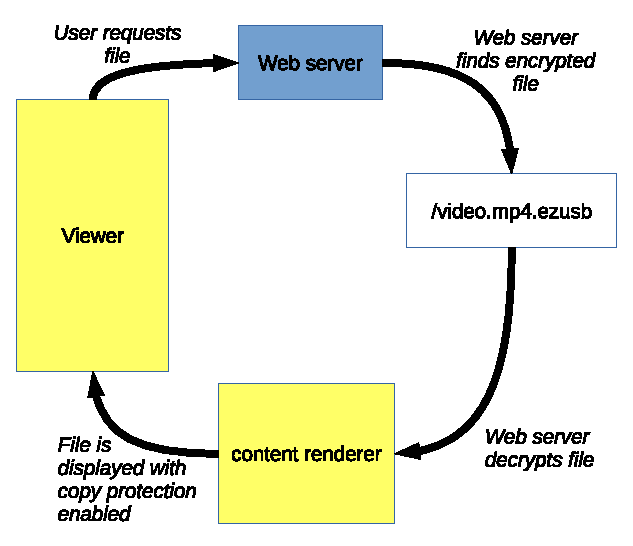
\includegraphics{contentloop.eps}
\label{fig:contentloop}
\end{figure}

To accomplish this, the system has two main parts: the \verb+FILESYSTEM+ 
and the \verb+WEBAPP+, as shown in Figure \ref{fig:mainmods}.

\begin{figure}
\centering
\caption{Main Modules}
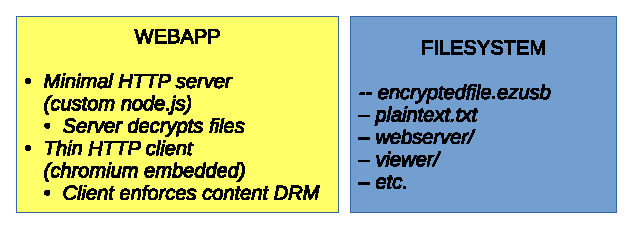
\includegraphics{mainmods.eps}
\label{fig:mainmods}
\end{figure}

\subsection{Filesystem \& Encryption}
Single files are encrypted using a unique symetric AES cypher, using a
key generated based on a combination of the following information:
\begin{itemize}
\item Device serial number 
\item Device firmware version
\item Global Salt 
\item Per-device nonce.  \emph{This must be stored in the code in an
      obfuscated manner.}
\end{itemize}
This key is stored in memory by the web server, and is used to decrypt
\verb+*.evusb+ files before serving them to the renderer.

An option for implementation is \verb+p3x-aes-folder+.

\subsection{Webapp}

The webapp is responsible for:
\begin{itemize}
\item Launching the web server when the device is attached to 
      a compatible computer.
\item Launching a browser (e.g. Chromium embedded), which will allow
      the end user to browse, view, and play content.
\item Decrypting content files
\item Displaying content files 
\end{itemize}

An option for implementation is \verb+electronJS+, which includes some 
integration with node and chromium embedded.

\subsection{Loader}

The content is locked to a specific device.  That means the system includes
a simple loader that will:
\begin{enumerate}
\item Read a device's serial number.
\item Generate a nonce
\item Store the obfuscated key on the device
\item Encrypt protected content
\item Load data to the device.
\end{enumerate}

\section{Use Cases}

\begin{enumerate}
\item Loading Content
    \begin{enumerate}
    \item Client provides content to Every USB.
    \item Every USB runs the {\bf Loader} to load the data.
    \item The {\bf Loader} iterates through each attached (blank) USB drive,
          encryptes the data based on the device's nonce and serial number,
          and copies the data.
    \end{enumerate}

\item Viewing Content
    \begin{enumerate}
    \item End user receives the USB drive (via postal mail, trade show 
          promotional material, or other means).
    \item End user inserts the drive into a compatible machine.  The 
          system will run automatically.  NOTE: this should not require
          any elevated priviledges to run.
    \item The system starts the web server, launches the viewer (chromium
          embedded), and presents the main menu.
    \item The end user selects content to view.
    \item If the end use opens the drive as a media storage device, and 
          copies a media file off of the drive, it is encrypted and not
          viewable using standard tools.
    \end{enumerate}

\end{enumerate}

\section{Potential Resources}
The following are open source libraries and projects which may be used in the
project, either as a foundation for work or as a guideline.
\begin{itemize}
\item \url{https://electronjs.org/}
\item \url{https://www.nodejs.org}
\item \url{https://www.npmjs.com/package/p3x-aes-folder}
\item \url{https://github.com/tessel/node-usb/tree/master/src}
\item \url{https://github.com/limpkin/mooltiapp} (For retrieving 
      firmware version and device IDs)
\item \url{http://janaxelson.com/hidpage.htm}
\item \url{https://github.com/kuscsik/chromiumembedded}
\end{itemize}

\end{document}
